\section{Control of the attitude of the system}
In this section a \emph{noninteracting} approach to the control of the
attitude of the system is introduced. The results of the simulations executed with
MATLAB Simulink are then presented.

\subsection{Noninteracting Control}
Noninteracting Control is defined as the problem of finding a feedback law in order
to reduce a multivariable system, from an input-output point of view, to a series of independent
single-input single-output channels. The following presentation is taken from Isidori \cite{Isidori1999}.
\par
The starting point is that of a nonlinear system in control affine form
\[
\vec{\dot{x}} = \vec{f}(\vec{x}) + \sum\limits_{i=1}^m \vec{g}_{i}(\vec{x}) u_{i}
\]
\[
y_{1} = h_{1}(\vec{x})
\]
\[
\hdots
\]
\[
y_{m} = h_{m}(\vec{x})
\]
and an initial point $\vec{x}^{0}$. Then the problem of noninteracting control is stated
as the problem of finding a static state feedback
\footnote{To be more precise the static state feedback should be \emph{regular}, i.e., the
  matrix $\beta(\vec{x})$ is nonsingular for all $x$.}
of the form
\begin{equation}\label{eq:nic_input}
  u_{i} = \alpha_{i}(\vec{x}) + \sum\limits_{j=1}^m \beta_{ij}(\vec{x})v_{j}
\end{equation}
defined in a neighborhood $U$ of $\vec{x}^{0}$ such that in the resulting closed loop system
\[
\vec{\dot{x}} = \vec{f}(\vec{x}) + \sum\limits_{i=1}^m \alpha_i(\vec{x}) +
\sum\limits_{j=1}^m\left(\sum\limits_{i=1}^m \vec{g}_i(\vec{x}) \beta_{ij}(\vec{x})\right)v_{j}
\]
\[
y_{1} = h_{1}(\vec{x})
\]
\[
\hdots
\]
\[
y_{m} = h_{m}(\vec{x})
\]
each output $y_i$ is affected only by the corresponding input $v_i$ and not by others.
\par
The main result \cite{Isidori1999} about the noninteracting control problem is the following.
\begin{prop}\label{prop:p1}
  Consider a multivariable nonlinear system with $m$ inputs and $m$ outputs
  \[
  \vec{\dot{x}} = \vec{f}(\vec{x}) + \sum\limits_{i=1}^m \vec{g}_{i}(\vec{x}) u_{i}
  \]
  \[
  y_{1} = h_{1}(\vec{x})
  \]
  \[
  \hdots
  \]
  \[
  y_{m} = h_{m}(\vec{x})
  \]
  Suppose
  \begin{equation}\label{eq:nic_prop_cond1}
    L{\vec{g}_j}L_{\vec{f}}^{k}h_{i}(\vec{x}) = 0 \quad 1 \le j \le m, \enspace 1 \le i \le m, \enspace k < r_i-1
  \end{equation}
  for all $\vec{x}$ in a neighborhood of $\vec{x}^{0}$ and
  \[
  \begin{bmatrix}
    L_{\vec{g}_1}L_{\vec{f}}^{r_{i-1}}h_i(\vec{x}^{0}) \enspace \hdots \enspace L_{\vec{g}_m}L_{\vec{f}}^{r_i-1}h_i(\vec{x}^{0})
  \end{bmatrix}
  \ne
  \begin{bmatrix}
    0 \enspace \hdots \enspace 0
  \end{bmatrix}
  \enspace 1 \le i \le m
  \]
  Then the noninteracting control problem is solvable if and only if the matrix
  \begin{equation}\label{eq:decoupling_matrix}
    \left[A(\vec{x})\right]_{ij} = a_{ij}(\vec{x}) = L_{\vec{g}_j}L_{\vec{f}}^{r_i-1}h_{i}(\vec{x})
  \end{equation}
  evaluated at the point $\vec{x}^{0}$ is nonsingular.
\end{prop}
The condition (\ref{eq:nic_prop_cond1}) and the non singularity of the matrix $A$
also correspond to the definition of a multivariable nonlinear system with a
\emph{vector relative degree} $\{r_1,\hdots,r_m\}$ at the point $\vec{x}^{0}$
and imply that $i$-$th$ output of the system has to be differentiated $r_i$ times
in order to have at least one component of the input vector $\vec{u}(t_0)$ explicitly
appearing at the time $t_0$ in which the state assumes the value
$\vec{x}^0$.
\par
In order to find the actual form of the controls (\ref{eq:nic_input}) the sufficiency
of the proposition (\ref{prop:p1}) is explained.
\par
First of all the system is written in a special form called \emph{normal form}
obtained using the following coordinates transformation
%% {\small
%%   \[
%%   \Phi(x) = [h_1(\vec{x}),\hdots,L_{\vec{f}}^{r_{i}-1}h_1(\vec{x}),\hdots,
%%     h_m(\vec{x}),\hdots,L_{\vec{f}}^{r_{m}-1}h_m(\vec{x}), \phi_{r+1}, ...,
%%     \hdots,\phi_{n}(\vec{x})]^{T}
%%   \]
%}
{\small
  \[
  \Phi(x) = [
    \phi_{1}^{1}(\vec{x}),\hdots,\phi_{r_{1}}^{1}(\vec{x}),
    \hdots,
    \phi_{1}^{m}(\vec{x}),\hdots,\phi_{r_{m}}^{m}(\vec{x}),
    \phi_{r+1}(\vec{x}),\hdots,\phi_{n}(\vec{x})
  ]
  \]
}
\[
\phi_{1}^{i}(\vec{x}) = h_{i}(\vec{x})
\]
\[
\phi_{2}^{i}(\vec{x}) = L_{\vec{f}}h_{i}(\vec{x})
\]
\[
\hdots
\]
\[
\phi_{r_{i}}^{i}(\vec{x}) = L_{\vec{f}}^{r_{i}-1}h_i(\vec{x})
\]
where $n$ is the dimension of the state $\vec{x}$ and $r = r_1 + \hdots + r_m$.
The fact that the system has a vector relative degree at $\vec{x}^{0}$ assures that
if $r < n$ it is always possible to find $n - r$ functions $\phi_{r+1},\hdots,\phi_{n}$
such that $\Phi(\vec{x})$ has a jacobian matrix which is nonsingular at $\vec{x}^{0}$
hence it can be used as a local coordinates transformation in a neighborhood of
$\vec{x}^{0}$. The new state is now defined as
\[
\vec{z} = \Phi(\vec{x}) =
\begin{bmatrix}
  \vec{\xi}\\
  \vec{\eta}
\end{bmatrix}
\]
where
\[
\vec{\xi} = [\left(\vec{\xi}^{1}\right)^T,\hdots, \left(\vec{\xi}^{m}\right)^T]^T
\]
\[
\vec{\xi}^{i} =
\begin{bmatrix}
  \xi_{1}^{i}\\
  \xi_{2}^{i}\\
  \vdots\\
  \xi_{r_{i}}^{i}
\end{bmatrix}=
\begin{bmatrix}
  h_{i}(\vec{x})\\
  L_{\vec{f}}h_i(\vec{x})\\
  \vdots\\
  L_{\vec{f}}^{r_{i}-1}h_i(\vec{x})
\end{bmatrix}
\]
and
\[
\vec{\eta} =
\begin{bmatrix}
  \phi_{r+1}(\vec{x})\\
  \phi_{r+2}(\vec{x})\\
  \vdots\\
  \phi_{n}(\vec{x})
\end{bmatrix}
\]
Using the definition of vector relative degree the time rate of change of $\vec{\xi}^{i}$ evaluates to
\[
\dot{\xi}_{1}^{i} = \xi_{2}^{i}
\]
\[
\hdots
\]
\[
\dot{\xi}_{r_{i}-1}^{i} = \xi_{r_{i}}^{i}
\]
\[
\dot{\xi}_{r_{i}}^{i} = b_{i}(\vec{\xi},\vec{\eta}) + \sum\limits_{j=1}^{m}a_{ij}(\vec{\xi},\vec{\eta})u_{j}
\]
for $1 \le i \le m$ where
\[
b_{i}(\vec{\xi},\vec{\eta}) = L_{\vec{f}}^{r_{i}}h_{i}(\Phi^{-1}(\vec{\xi},\vec{\eta}))
\enspace 1 \le i \le m
\]
and
\[
a_{ij}(\vec{\xi},\vec{\eta}) = L_{\vec{g}_j}L_{\vec{f}}^{r_i-1}h_{i}(\Phi^{-1}(\vec{\xi},\vec{\eta}))
\enspace 1 \le i,j \le m
\]
is the same as defined in (\ref{eq:decoupling_matrix}) but evaluated in $\vec{x} = \Phi^{-1}(\vec{\xi},\vec{\eta})$.
As regards the remaining part of the new coordinates $\vec{\eta}$ only a generic equation of the form
\[
\vec{\dot{\eta}} = \vec{q}(\vec{\xi},\vec{\eta}) + \vec{p}(\vec{\xi},\vec{\eta})\vec{u}
\]
can be stated for some vector valued functions $\vec{q}$ and $\vec{p}$.
\par
Collecting the coefficients $b_i(\vec{\xi},\vec{\eta})$ in a vector
$\vec{b}(\vec{x})$ evaluated at $\vec{x} = \Phi^{-1}(\vec{\xi},\vec{\eta})$
then the vector containing the higher order derivatives of each output can be
written as
\[
\begin{bmatrix}
  \dot{\xi}_{r_{1}}^{1}\\
  \vdots\\
  \dot{\xi}_{r_{m}}^{m}\\
\end{bmatrix}=
\vec{b}(\vec{\xi},\vec{\eta}) + A(\vec{\xi},\vec{\eta})\vec{u}
\]
If now a feedback law of the form
\[
\vec{u} = -A^{-1}(\vec{\xi},\vec{\eta})\vec{b}(\vec{\xi},\vec{\eta}) + A^{-1}(\vec{\xi},\vec{\eta})\vec{v}
\]
is selected one obtains
\[
\begin{split}
  \begin{bmatrix}
    \dot{\xi}_{r_{1}}^{1}\\
    \vdots\\
    \dot{\xi}_{r_{m}}^{m}\\
  \end{bmatrix}=&
  \vec{b}(\vec{\xi},\vec{\eta}) + A(\vec{\xi},\vec{\eta})
  (-A^{-1}(\vec{\xi},\vec{\eta})\vec{b}(\vec{\xi},\vec{\eta}) + A^{-1}(\vec{\xi},\vec{\eta})\vec{v})\\
  =&
  \vec{b}(\vec{\xi},\vec{\eta})-\vec{b}(\vec{\xi},\vec{\eta}) + \vec{v}
  = \vec{v}
\end{split}
\]
In summary the closed loop system is characterized by the $m$ sets of equations
\[
\dot{\xi}_{1}^{i} = \xi_{2}^{i}
\]
\[
\hdots
\]
\[
\dot{\xi}_{r_{i}-1}^{i} = \xi_{r_{i}}^{i}
\]
\[
\dot{\xi}_{r_{i}}^{i} = v_{i}
\]
\[
y_{i} = \xi_{1}^{i}
\]
for $1 \le i \le m$, together with
\[
\begin{split}
  \vec{\dot{\eta}} =& \vec{q}(\vec{\xi},\vec{\eta})
  -\vec{p}(\vec{\xi},\vec{\eta})A^{-1}(\vec{\xi},\vec{\eta})\vec{b}(\vec{\xi},\vec{\eta})
  +\vec{p}(\vec{\xi},\vec{\eta})A^{-1}(\vec{\xi},\vec{\eta})\vec{v}\\
  =&\hat{\vec{q}}(\vec{\xi},\vec{\eta}) + \hat{\vec{p}}(\vec{\xi},\vec{\eta})\vec{v}
\end{split}
\]
As shown in the block diagram in Figure \ref{fig:nic_diagram}
\begin{figure}[h]
  \centering
  \includegraphics[scale=0.13]{nic_diagram}
  \caption{Noninteractive control block diagram \label{fig:nic_diagram}}
\end{figure}
each input $v_{i}$ controls only the output $y_{i}$ through a chain of
$r_{i}$ integrators as required by the noninteractive control problem.
If $r = r_{1} + \hdots + r_{m} < n$ the closed loop system also has an unobservable
part which is affected by all inputs and all states but does not affect the outputs.
\par
Reverting back to the original set of coordinates of the system the feedback law
results
\[
\vec{u} = \vec{\alpha}(\vec{x}) + \beta(\vec{x})\vec{v}
\]
where
\[
\vec{\alpha}(\vec{x}) = -A^{-1}\vec{b}(\vec{x})\qquad \beta(\vec{x}) = A^{-1}(\vec{x})
\]
This form of feedback is also called \emph{Standard Noninteractive Feedback} and in general
is defined only \emph{locally} in the state space, i.e., for all $\vec{x}$ near $\vec{x}^0$
at which the matrix $A(\vec{x})$ is nonsingular.

\subsection{Application of the noninteractive feedback}
Consider the system (\ref{eq:nl_eq_2})
\[
\begin{split}
  \dot{\vec{x}} &= \vec{f}(\vec{x}) + g(\vec{x})\vec{u}\\
  &=\vec{f}(\vec{x}) +
  \begin{bmatrix}
    0_{3\times3} \\
    \left(B(\theta_2,\theta_3) ^ {-1}\right)_{(:, 4:6)}
  \end{bmatrix}\vec{u}\\
\end{split}
\]
with outputs given in eq. (\ref{eq:output})
\[
\vec{y} = \vec{h}(\vec{x}) =
\begin{bmatrix}
  \theta_1 &
  \theta_2 &
  \theta_3
\end{bmatrix}^T
\]
The purpose of this section is to assess whether, by means of a feedback of the form
(\ref{eq:nic_input}), a closed loop system in which each angle $\theta_i$ is controlled
independently of others can be obtained. If this is possible than the final aim is to obtain
a second order dynamics of the form
\begin{equation}\label{eq:des_dynamics}
\ddot{\theta}_{i} = \ddot{\theta}^{des}_{i} + k_d (\dot{\theta}^{des}_{i} - \dot{\theta}_{i}) + k_p (\theta^{des}_{i} - \theta_{i})
\end{equation}
where $\ddot{\theta}^{des}_{i}$, $\dot{\theta}^{des}_{i}$ and $\theta^{des}_{i}$ are
the desired trajectories.
\par
In order to apply the noninteracting control approach to the system it is required to
verify if the system has a vector relative degree at some point $\vec{x}^0$ in the state space.
Simple calculations
\[
L_{\vec{g}_{j}}L_{\vec{f}}^{0}h_{i} =
L_{\vec{g}_{j}}h_{i} = 
\begin{bmatrix}
  \vec{e}_i & 0_{6x1}
\end{bmatrix}
\vec{g}_j
=
g_{j}^{i} = 0
\qquad 1 \le j \le 3, \enspace 1 \le i \le 3
\]
show that the condition (\ref{eq:nic_prop_cond1}) is verified for every $\vec{x}$ in the state space.
Also the second derivative of the output with respect to time can be written as
\[
\frac{\mathrm{d}^{2}}{\mathrm{d}t^{2}}\vec{y} = 
\begin{bmatrix}
  \ddot{\theta_1}\\
  \ddot{\theta_2}\\
  \ddot{\theta_3}
\end{bmatrix} =
\vec{b}(\vec{x}) + A(\vec{x}) \vec{u}
\]
where
\[
\vec{b}(\vec{x}) = \vec{f}(\vec{x})_{(4:6)}
\]
and
\[
A(\vec{x}) = \left(B(\theta_2,\theta_3) ^ {-1}\right)_{(1:3, 4:6)}
\]
As shown in figure \ref{fig:detA} the determinant of the matrix $A$ is nonzero
\begin{figure}[h]
  \centering
  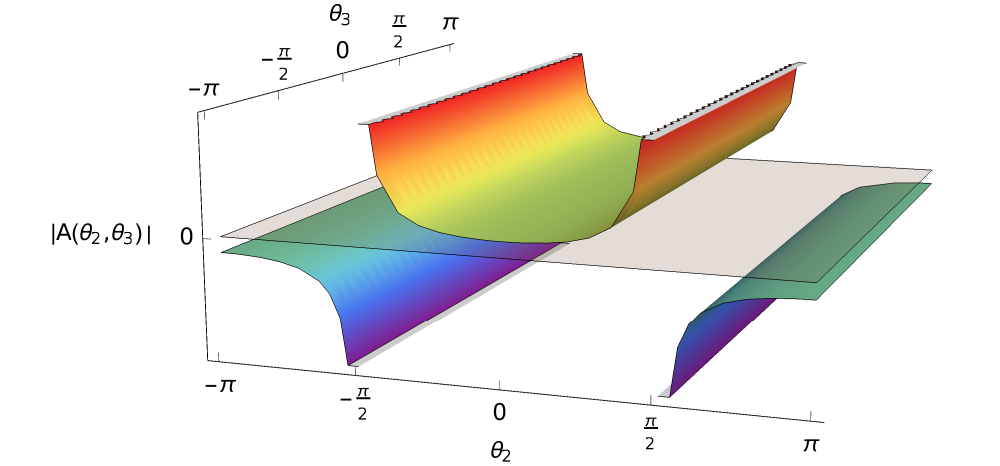
\includegraphics[scale=0.5]{detA}
  \caption{Determinant of the decoupling matrix A \label{fig:detA}}
\end{figure}
for every $\theta_2$ and $\theta_3$ hence the system has a vector
relative degree $\{2,2,2\}$ everywhere. The resulting standard noninteractive feedback
is
\[
\vec{u}_{NIC} = -\left(B(\theta_2,\theta_3) ^ {-1}\right)_{(1:3, 4:6)}^{-1}
(\vec{f}_{(4:6)}(\vec{x}) - \vec{v} )
\]
where $\vec{v}$ can be chosen as
\begin{equation}\label{eq:PD}
v_i(\theta_i, \dot{\theta_i}) = \ddot{\theta}^{des}_{i} + k_d (\dot{\theta}^{des}_{i} - \dot{\theta}_{i}) + k_p (\theta^{des}_{i} - \theta_{i})
\end{equation}
in order to obtain the desired closed loop dynamics (eq. \ref{eq:des_dynamics}).
\subsubsection{Unobservable part of the system}
In order to write the equations of the unobservable part of the closed
loop system the coordinate transformation $\Phi$ must be specified entirely.
The choice of the outputs
\[
\vec{y} = \vec{h}(\vec{x}) =
\begin{bmatrix}
  \theta_1 &
  \theta_2 &
  \theta_3
\end{bmatrix}^T
\]
implies
\[
\phi_1 (\vec{x}) = \theta_1 \quad \phi_3 (\vec{x}) = \theta_2 \quad \phi_5 (\vec{x}) = \theta_3
\]
\[
\phi_2 (\vec{x}) = \dot{\theta}_1 \quad \phi_4 (\vec{x}) = \dot{\theta}_2 \quad \phi_6 (\vec{x}) = \dot{\theta}_3
\]
The remaining $3$ functions $\phi_7(\vec{x})$, $\phi_8(\vec{x})$ and $\phi_9(\vec{x})$ are chosen to be the last
three components of the state
\[
\phi_7(\vec{x}) = x_7 = \dot{q}_x \quad \phi_8(\vec{x}) = x_8 = \dot{q}_y
\quad \phi_9(\vec{x}) = x_9 = \dot{q}_z
\]
The resulting mapping $\Phi(\vec{x})$ has a jacobian
\[
\frac{\partial \Phi(\vec{x})}{\partial \vec{x}} =
%% \begin{bmatrix}
%%   1 & 0 & 0 & 0 & 0 & 0 & 0 & 0 & 0\\
%%   0 & 0 & 0 & 1 & 0 & 0 & 0 & 0 & 0\\
%%   0 & 1 & 0 & 0 & 0 & 0 & 0 & 0 & 0\\
%%   0 & 0 & 0 & 0 & 1 & 0 & 0 & 0 & 0\\
%%   0 & 0 & 1 & 0 & 0 & 0 & 0 & 0 & 0\\
%%   0 & 0 & 0 & 0 & 0 & 1 & 0 & 0 & 0\\
%%   0 & 0 & 0 & 0 & 0 & 0 & 1 & 0 & 0\\
%%   0 & 0 & 0 & 0 & 0 & 0 & 0 & 1 & 0\\
%%   0 & 0 & 0 & 0 & 0 & 0 & 0 & 0 & 1\\
%% \end{bmatrix}
\begin{bmatrix}
  \vec{e}_{1} & \vec{e}_{3} & \vec{e}_{5} & \vec{e}_{2} & \vec{e}_{4} & \vec{e}_{6} &
  \vec{e}_{7} & \vec{e}_{8} & \vec{e}_{9}
\end{bmatrix}
\]
which is nonsingular and hence can be used
as coordinate transformation everywhere.
\par
The dynamics of the unobservable part of the closed loop system, i.e.,
of the flywheels, can be written as
\[
\begin{split}
\dot{\vec{\eta}} &=
\begin{bmatrix}
  \ddot{q}_{x}\\
  \ddot{q}_{y}\\
  \ddot{q}_{z}
\end{bmatrix}
= \vec{f}_{(7:9)}(\vec{x}) + \left(B(\theta_2,\theta_3) ^ {-1}\right)_{(4:6, 4:6)} \vec{u}_{NIC}\\
&=\vec{f}_{(7:9)}(\vec{x}) - \left(B(\theta_2,\theta_3) ^ {-1}\right)_{(4:6, 4:6)}
\left(B(\theta_2,\theta_3) ^ {-1}\right)_{(1:3, 4:6)}^{-1}
(\vec{f}_{(4:6)}(\vec{x}) - \vec{v})\\
&=\hat{\vec{q}}(\vec{x}) + \hat{\vec{p}}(\theta_{2},\theta_{3})\vec{v}
\end{split}
\]

\subsection{Results of simulation}
In the following figures the results of the simulation done
in MATLAB Simulink are presented.
The desired trajectory was chosen as
\[
\theta_1^{des}(t) = a_0 + a_1 t + a_2 t^2 + a_3 t^3 + a_4 t^4 + a_5 t^5
\]
with boundary conditions
\[
\begin{split}
  %% &\theta_1^{des}(0) \in [-\pi, \pi) \quad \dot{\theta}_1^{des}(0)= 0 \quad \ddot{\theta}_1^{des}(0) = 0\\
  %%   &\theta_1^{des}(t_{f}) \in [-\pi, \pi)  \quad \dot{\theta}_1^{des}(t_{f})= 0 \quad \ddot{\theta}_1^{des}(t_{f}) = 0
  &\theta_1^{des}(0) = 0 \quad \dot{\theta}_1^{des}(0)= 0 \quad \ddot{\theta}_1^{des}(0) = 0\\
    &\theta_1^{des}(t_{f}) = \pi \quad \dot{\theta}_1^{des}(t_{f})= 0 \quad \ddot{\theta}_1^{des}(t_{f}) = 0
\end{split}
\]
and
\[
\theta_2^{des}(t) \equiv -\mathrm{atan}\frac{\sqrt{2}}{2}
\]
\[
\theta_3^{des}(t) \equiv \frac{\pi}{4}
\]
Such a trajectory corresponds to a rotation about the $z$ axis of the inertial
reference frame $\{S\}$ while the balance on one of the corner is maintained.
The resulting control law is
\begin{equation}\label{eq:PD_yaw}
  \begin{split}
    &v_1(t) = \ddot{\theta}_1^{des}(t) + k_d(\dot{\theta}_1^{des}(t) - \dot{\theta}_1(t)) + k_p (\theta_1^{des}(t) - \theta_1(t))\\
    &v_2(t) = - k_d\dot{\theta}_2(t) + k_p \left(-\mathrm{atan}\frac{\sqrt{2}}{2} - \theta_2(t)\right)\\
    &v_3(t) = - k_d\dot{\theta}_3(t) + k_p \left(\frac{\pi}{4} - \theta_3(t)\right)
  \end{split}
\end{equation}
%% It should be noted that the initial state $\vec{x}(0)$ and the final state $\vec{x}(t_{f})$
%% corresponding to the desired trajectory belong to the set of equilibria $\mathcal{E}_{1}$ provided that
%% the velocities of the flywheels are zero in $t=0$ and $t=t_{f}$.
\par
In figure \ref{fig:orientation_error} the orientation error is shown while
in figure \ref{fig:requested_torques} the required torques are shown.
\begin{table}[h]
  \begin{tabular}{cc}
    \begin{subfigure}{0.5\textwidth}
      \centering
      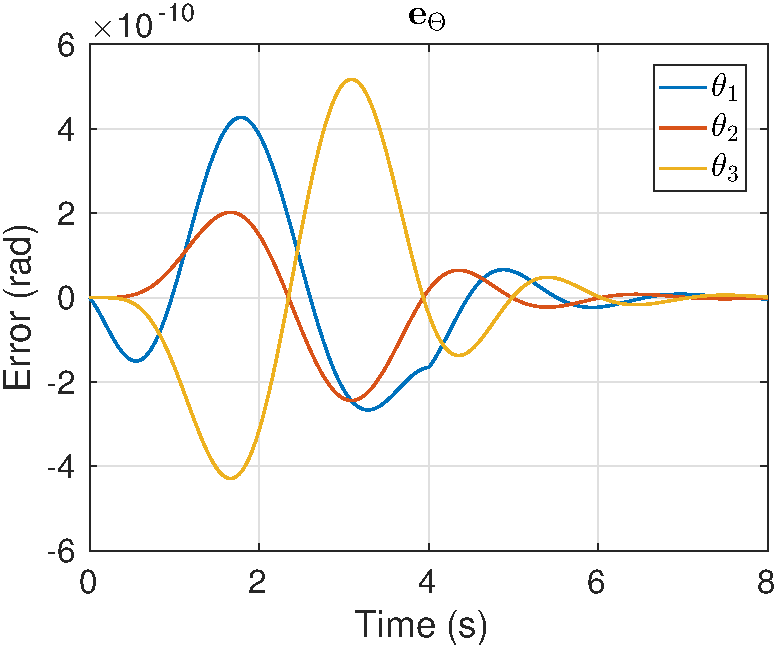
\includegraphics[scale=0.5]{error}
      \caption{Orientation error \label{fig:orientation_error}}
    \end{subfigure}&
    \begin{subfigure}{0.5\textwidth}
      \centering
      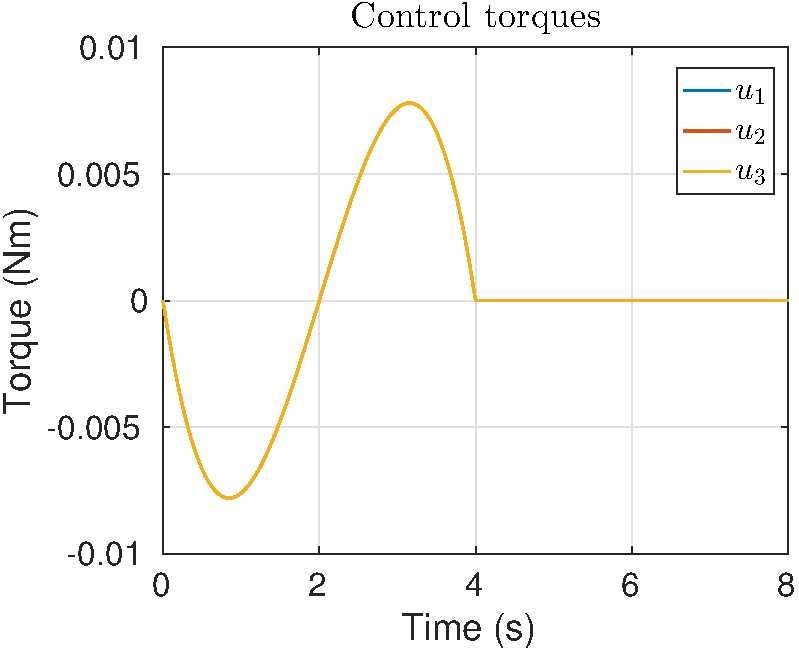
\includegraphics[scale=0.5]{input}
      \caption{Control torques \label{fig:requested_torques}}
    \end{subfigure}
  \end{tabular}
  \caption{Results of simulation ($k_p = 10$, $k_d = 0.1$)}
\end{table}

%% \clearpage
\subsubsection{Steady state behavior of the unobservable subsystem}
As shown in the figure \ref{fig:fw_velocites} the
flywheel velocities $\vec{\eta}(t)$ which are solution to the differential
equation
\[
\begin{cases}
\dot{\vec{\eta}} = \hat{\vec{q}}(\vec{x}) + \hat{\vec{p}}\left(-\mathrm{atan}\frac{\sqrt{2}}{2},\frac{\pi}{4}\right)\vec{v}\\
\vec{\eta}(0) = \vec{0}
\end{cases}
\]
with $\vec{v}$ given in (\ref{eq:PD_yaw}) are bounded and tends to zero.
\begin{figure}[h]
  \centering
  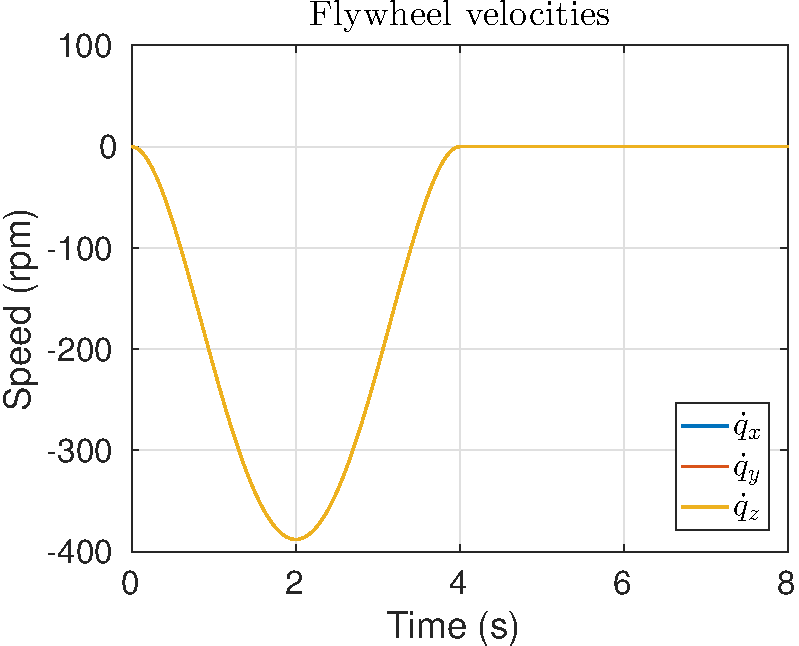
\includegraphics[scale=0.7]{fly_wheel}
  \caption{Flywheel velocities ($k_p = 10$, $k_d = 0.1$)\label{fig:fw_velocites}}
\end{figure}

\subsubsection{Use of an alternative Euler parametrization}
In this section the results of the same simulation obtained using a different parametrization of the rotation matrix
$R_{SC}$, i.e. Euler XYZ instead of Euler ZYX, are presented. The theory described up to now
can be still applied with the exception that the rotation of the cubic frame around the $z$ axis
of the intertial reference frame $\{S\}$ cannot be mapped to a single angle. Instead all three angles
have to change and the intermediate poses of the frame, which determine the desired trajectory, can be found 
using a spherical linear interpolation approach (Slerp). Using this set-up however the simulations reveal that
the velocites of the flywheels reamain non-zero but constant at the end of the rotation. In other words
the state $\vec{\eta}$ of the unobservable part of the closed loop system subjected to the new slerp-based input does not
tend to zero. Altough impractical in a real implementation this behavior is compatible with the existence of
equilibria in which the system is at rest in the upright position while the flywheels rotates at a non zero constant angular velocity.
\par
A possible solution to slow down the flywheel velocities is to switch to a LQR based control after the rotation
is completed. Such a controller should be synthesized using the linear approximation of the system around an equilibrium
point where the system is at rest in the upright position with zero flywheel velocities. Extensive simulations show that
the linear approximation around such equilibrium points is always stabilizable. However there are cases in which
the flywheel velocities before the switching are too high and the state of the system is out of the region
of attraction of the LQR controller.
\par
In the figures below an example of the described approach is presented.
The desired trajectory and the NIC controller allow to rotate the cubic frame
by an angle of $\pi$ in $\SI{4}{\second}$ with zero steady state error. As can be
seen from figure \ref{fig:fw_velocites_lqr} the flywheel velocities reamain non-zero
but constant after the rotation. At time $t=\SI{5}{\second}$ the LQR controller is
actived and the flywheel velocities tends to zero asymptotically.
\begin{table}[h]
  \begin{tabular}{cc}
    \begin{subfigure}{0.5\textwidth}
      \centering
      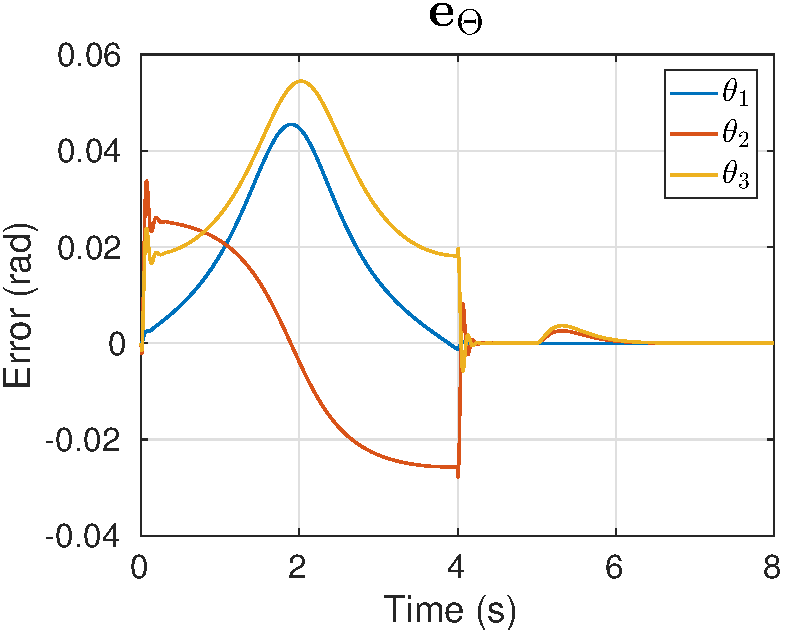
\includegraphics[scale=0.5]{error_lqr}
      \caption{Orientation error \label{fig:orientation_error_lqr}}
    \end{subfigure}&
    \begin{subfigure}{0.5\textwidth}
      \centering
      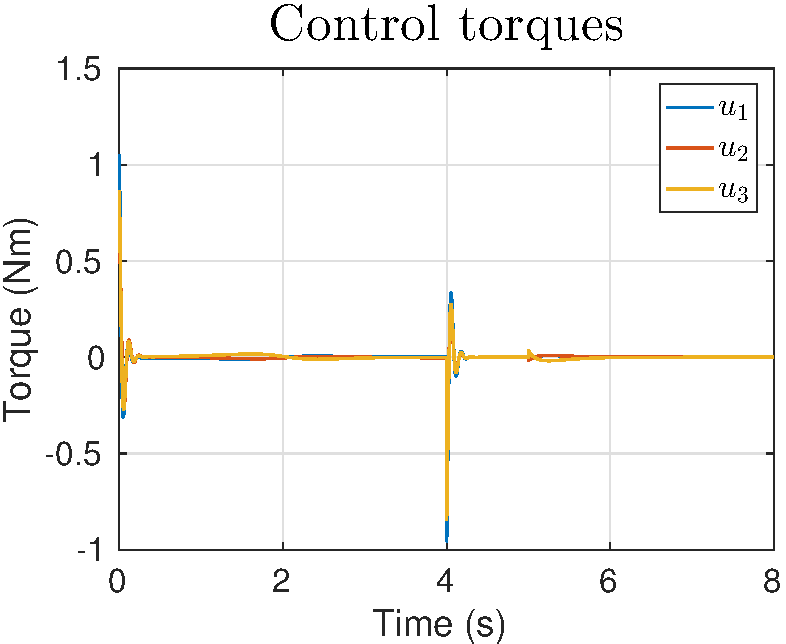
\includegraphics[scale=0.5]{input_lqr}
      \caption{Control torques \label{fig:requested_torques_lqr}}
    \end{subfigure}
  \end{tabular}
  \caption{Results of simulation ($k_p = 2500$, $k_d = 50$)}
\end{table}
\begin{figure}[h]
  \centering
  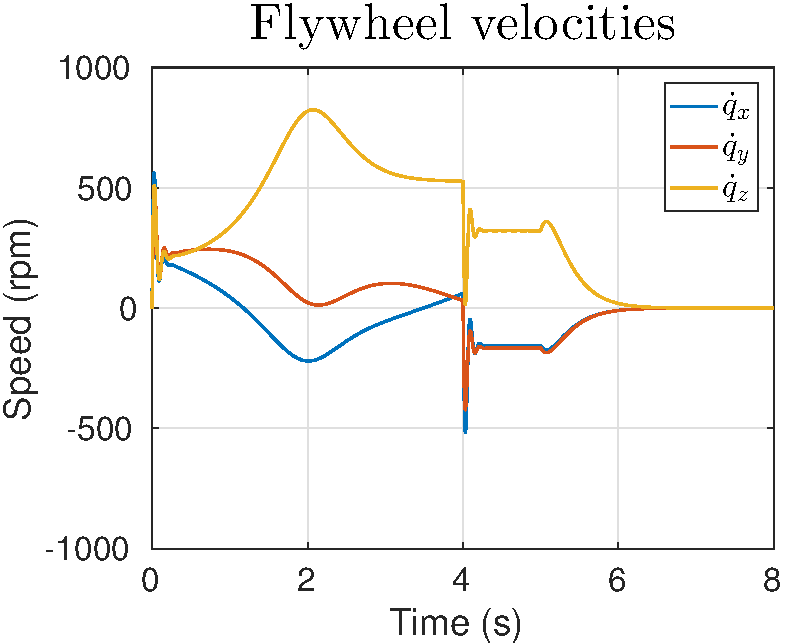
\includegraphics[scale=0.6]{fly_wheel_lqr}
  \caption{Flywheel velocities ($k_p = 2500$, $k_d = 50$)\label{fig:fw_velocites_lqr}}
\end{figure}
\par
In the figure \ref{fig:simulation_lqr} the outcome of the switch to the LQR controller
is shown for several angles of rotation and several durations of the movement.
\begin{figure}[h]
  \centering
  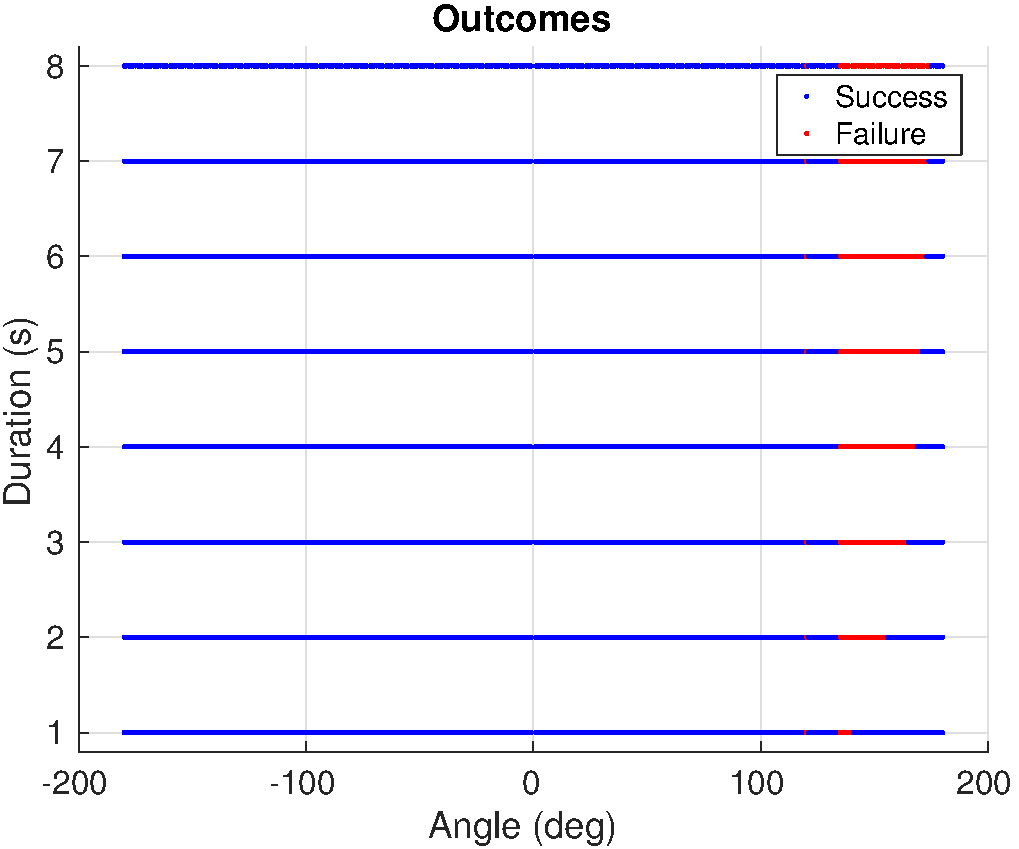
\includegraphics[scale=0.46]{simulation_lqr}
  \caption{Outcome of the switch to LQR\label{fig:simulation_lqr}}
\end{figure}
In the figure \ref{fig:simulation_lqr_velocities} it is shown that
the failures happen when the flywheel velocities are too high.
\begin{figure}[h]
  \centering
  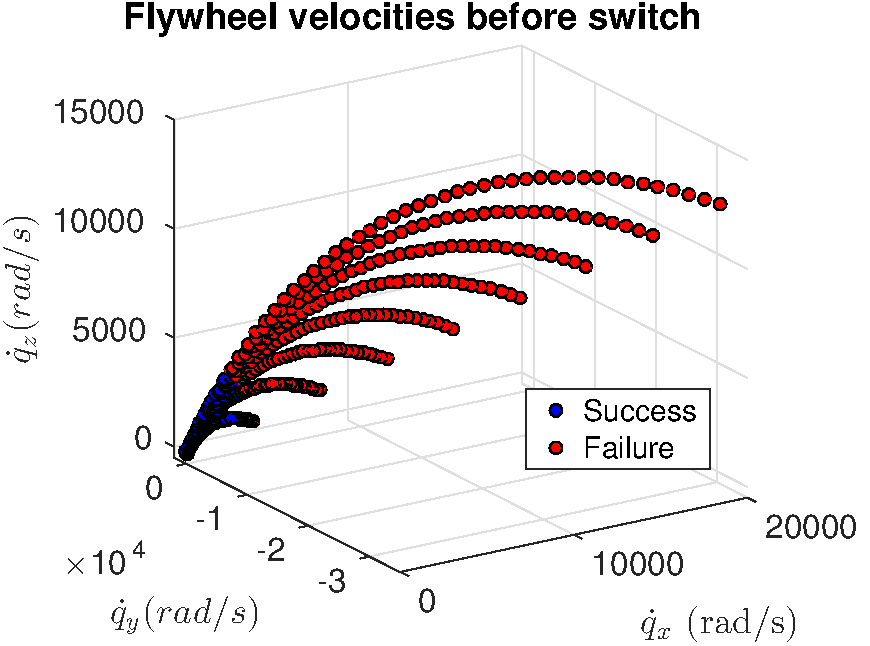
\includegraphics[scale=0.62]{simulation_lqr_velocities}
  \caption{Flywheel velocities before the switch to LQR\label{fig:simulation_lqr_velocities}}
\end{figure}

\newpage
